\chapter{Background}
The second chapter, \textit{Background}, explains the background necessary to understand the Bachelor thesis. 
In the first section, \textit{Definitions}, terms are defined that are used in this Bachelor thesis.
The second section, \textit{Methodology}, presents the methodology applied to analyse the problem of finding a parked car and used to improve the user interface design.
In the third section, \textit{Related Systems}, applications for iOS\footnote{iOS: \url{https://www.apple.com/ios/ios-13/}, (online: last accessed October 19, 2019)} are presented, that solve the problem of finding a parked car.
In the fourth section, \textit{Related Work}, academic work that relates to the bachelor thesis is discussed.

\section{Definitions}

\paragraph{Spatial Trajectory} A spatial trajectory is a trace of an object through a geographical space. It is usually represented as a chronologically ordered list of points $ P = p_1\rightarrow p_2 \rightarrow \dots \rightarrow p_n$. The points consist of a geospatial coordinate set and a timestamp $p_i=(lat,lon,t)$. \cite{Zheng:2015:TDM:2764959.2743025}

\paragraph{Semantic Trajectory} A semantic trajectory is defined as a finite spatial trajectory with a semantic meaning, i.e. the used transportation mode $((p_1\rightarrow p_2 \rightarrow \dots \rightarrow p_n), label)$. \cite{Zheng:2015:TDM:2764959.2743025}

\paragraph{Trajectory Segmentation} In trajectory segmentation, a trajectory is divided into fragments by a measure such as time, spatial shape, or semantic meaning. These fragments can be used for further processing such as classification. \cite{Zheng:2015:TDM:2764959.2743025}

\paragraph{Trajectory Classification} The process of predicting the class label of trajectories, or their segments, based on their features is called trajectory classification. \cite{lee2008traclass}

\paragraph{Stay Point} A stay point $s$ is defined as a geographical location in which a user stays over a threshold time $T_r$ within a threshold distance $D_r$. In a spatial trajectory, a stay point $s$ is characterised by a set of consecutive points $P=p_m \rightarrow p_{m+1} \rightarrow \dots \rightarrow p_n$ with $\forall m<i\leq n:\: Dist(p_m, p_i) \leq D_r$, $Dist(p_m, p_{n+1}) > D_r $, and $t(p_n) - t(p_m) \geq T_r$. The stay point $s$ is then defined by $s=(lat, lon, t_a, t_l)$ where $lat(s) = \sum^{n}_{i=m}lat(p_i) /|P|$, $lon(s) = \sum^{n}_{i=m}lon(p_i)/|P|$, $t_a(s) = t(p_m)$, and $t_l(s) = t(p_n)$. \cite{Zheng2007}

\paragraph{Segment} A segment is defined as the edge between any two consecutive points in a spatial trajectory. In a spatial trajectory $P=p_1 \rightarrow \dots \rightarrow p_n$, each edge $p_i\rightarrow p_{i+1}, 1\leq i < n$ is called a segment. \cite{Zheng:2015:TDM:2764959.2743025}

\paragraph{Trip} A trip $T_i$ is defined as the subset of a spatial trajectory between two consecutive stay points. $T_i = \{p \in P |\: s_i.l \leq p.t \leq s_{i+1}.a \}$, where $T_i$ is the set of all spatial trajectories of a trip, $P$ is the set of all recorded spatial trajectories of a user, and $s_i, s_{i+1}$ are two consecutive stay points of the user. The index $i$ is a natural number greater or equal zero.  \cite{Zheng2008}

\paragraph{Stage} A stage is a group of successive segments of the same transportation mode within a trip. A new stage starts where the transportation mode changes to another, or where the used vehicle is changed. \cite{Bolbol2012}

\paragraph{Transportation Mode} The transportation mode is the way in which an object moves through a space, such as walking, via car or via bus.  \cite{Bolbol2012}


\paragraph{Change Point} A change point is defined as the location where the transportation mode of a trajectory changes within a trip. \cite{Zheng2008}

\paragraph{Global Positioning System Standard Positioning Service} The Global Positioning System Standard Positioning Service is a positioning and timing service. It uses ranging signals transmitted by satellites. The signals contain a  coarse/acquisition (C/A)  code  ranging  signal and a navigation data message. 
\cite{dod2008global}


\paragraph{Precision} In the context of machine learning, the precision is the number of correctly positive labeled instances divided by the sum of the correctly positive labeled instances and the wrongly positive labeled instances. \cite{davis2006relationship}

\paragraph{Recall} The recall is the number of correctly positive labeled instances divided by the sum of the correctly positive labeled instances and the wrongly negative labeled instances. \cite{davis2006relationship}

\paragraph{F1-Score} The F1-score, also called the F-measure, is the harmonic mean of precision and recall. It is defined as $f_1 = (2 \cdot precision \cdot recall) / (precision + recall)$. \cite{sasaki2007truth}


\section{Methodology}

Four people are interviewed for background interviews. The goal of these interviews is to gain insight into the ''needs and expectations of users''. The interviews are performed using a semi-structured interview technique. In semi-structured interviews, the interviewer has a list of questions and the interviewee is encouraged to elaborate their answers. The interviewer can ask follow-up questions if more insight into a specific answer is needed. This technique is used because the detailed answers of the users allow insight into their expectations of the application and the option for asking follow-up questions avoids imprecise answers. A structured technique would not allow the users to mention their own expectations and issues. An unstructured technique would make the answers of the interviewees difficult to compare. The answers given in the interviews are summarised. Based on the results of the interviews and the limitations of this Bachelor thesis, requirements for the application are defined. The requirements are separated into functional and non-functional requirements. \cite{Abras2004} \cite{wilson2013interview}

To ensure the usability of the application, the user interface is created iteratively. Best practises are applied by using design heuristics by Nielsen and conforming to the Human Design Guidelines by Apple Inc\footnote{Apple Inc: \url{https://www.apple.com/} (online: last accessed October 19, 2019)}. Iterative design is defined as ''progressive refinement through cyclical data-driven development''. During each iteration, users test the current design prototypes. For these tests, the Think-Aloud method is applied. Think-Aloud is ''a special kind of verbal protocol in which the user says out loud what she is thinking while she is carrying out a task or doing some problem solving''. The method is chosen because it can lead to less design interactions while still resulting in efficient systems that are accepted by users. In the tests themselves, a prototype of the user interface is provided to the users. The users are asked to perform five different actions in the prototype and thereby think aloud. First, they are asked to determine the parking position of their car. Second, they are asked to use the navigation to find to their car. Third, they are asked to imagine their car is parked in a multi-storey parking lot and to answer how the application would help them to find their car in this scenario. Fourth, the users are asked to report the accuracy of the determined parking position. Fifth, they are asked to refresh the determined parking position. They are encouraged to elaborate what they are thinking and reasoning while using the prototype. After the tests are conducted, the protocols of the tests are analysed for potential obstacles in the user interface. The results are aggregated and summarised. The obstacles in the user interface are removed in the next iteration. The tests are repeated with the next prototype to ensure the changes have a positive impact on the usability of the application. \cite{Abras2004} \cite{goodman2012observing} \cite{nielsen1994usability} \cite{heurisitcNielsen} \cite{apple:interfaceguidliines} \cite{jaspers2004think} 

\section{Related Systems}

Apple Maps\footnote{Apple Maps, \url{https://www.apple.com/ios/maps/}, (online: last accessed October 19, 2019)}, which is preinstalled on iOS devices, supports the determination of the parking position of a car on an iPhone. The parking position is determined via the phone's connection to the car. When the Bluetooth connection or the CarPlay\footnote{CarPlay: \url{https://www.apple.com/ios/carplay/} (online: last accessed October 19, 2019)} connection, a proprietary way to connect cars with an iPhone, is interrupted, the phone logs the current position as the parking position of the car. The user can manually change and optimise the logged position, which can be seen in Figure \ref{fig:ios_park_det}, and add a photo to the saved location to simplify the process of finding the car. The approach used by Apple Maps is usable by users who connect their phone to their car regularly. It is not usable by users who either do not or cannot connect their phone to their car as there is no alternative solution for these users in Apple Maps. \cite{apple:maps:parkedcar}

\begin{figure}[h]
  \centering
  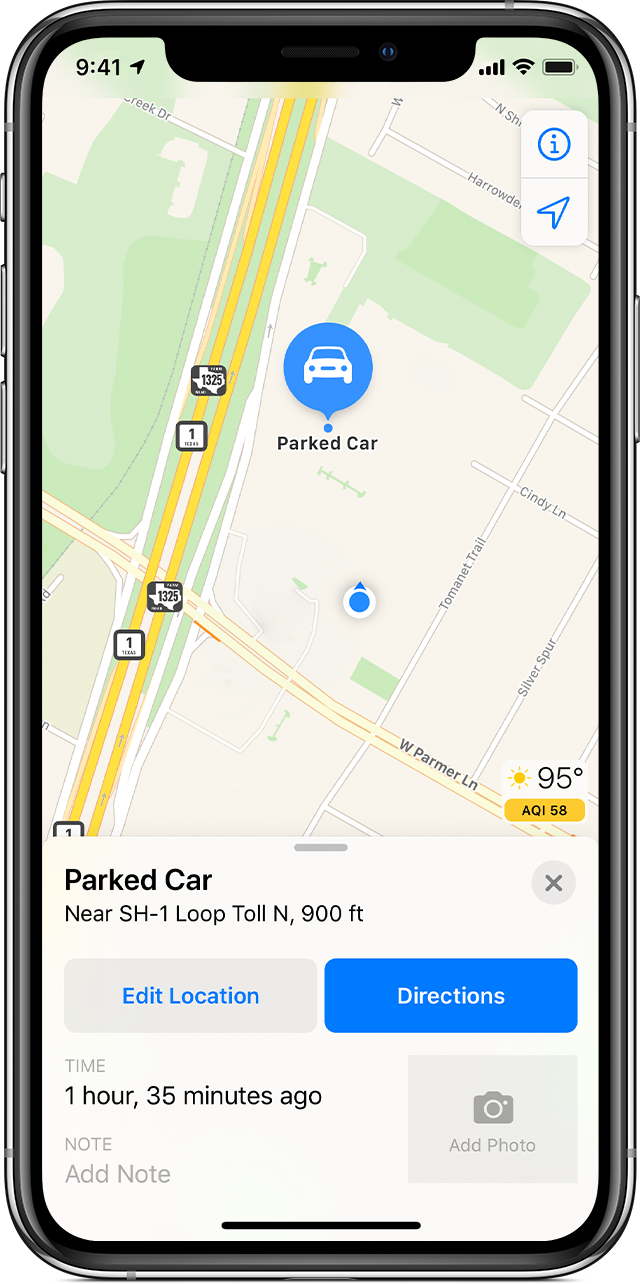
\includegraphics[width=0.3\textwidth]{images/ios13-iphone-xs-maps-parked-car.png}
  \caption{Apple Maps Parked Car, Image from Apple Support Page: \url{https://support.apple.com/en-us/HT207227} (online: last accessed October 19, 2019)}
  \label{fig:ios_park_det}
\end{figure}

Google Maps\footnote{Google Maps, \url{https://apps.apple.com/us/app/google-maps-transit-food/id585027354}, (online: last accessed October 19, 2019)} also offers the feature to determine the parking position of a user's car on an iPhone. Three different approaches are implemented. First,  the application can determine the parking position automatically via the motion and fitness activity data of the user. The used process for the determination via the Motion and Fitness Activity data is not public. The mentioned motion and fitness activity data include data from the iPhone`s accelerometer, gyroscope and magnetometer. The second approach is, similar to Apple Maps, based on the phone's connection to the user's car. The third approach is to let the user manually set the parking location. For this, the user taps their location on the map view and chooses to set the current position as parking location. Also, at the end of a navigation, the user can select their current position to be saved as parking position of their car. As Google Maps does not rely solely on the direct connection of the phone to the car, it is usable by any user, independent from the user's willingness or possibility to connect their phone to their car. \cite{google:maps:app:parkedcar}  \cite{apple:CoreMotion}

There are several application n the Apple AppStore\footnote{Apple AppStore, \url{https://www.apple.com/ios/app-store/}, (online: last accessed October 19, 2019)} which are dedicated to finding the parked car of the user. Find my Parked Car\footnote{Find my Parked Car, \url{https://apps.apple.com/us/app/find-my-parked-car/id987712319}, (online: last accessed October 19, 2019)}, Find My Car - Car Locator\footnote{Find My Car - Car Locator, \url{https://apps.apple.com/us/app/find-my-car-car-locator/id1295565906}, (online: last accessed October 19, 2019)}, Find My Car - GPS Auto Parking Reminder \& Tracker\footnote{Find My Car - GPS Auto Parking Reminder \& Tracker, \url{https://apps.apple.com/us/app/find-my-car-gps-auto-parking-reminder-tracker/id815542507}, (online: last accessed October 19, 2019)} and ParKing P\footnote{ParKing P, \url{https://apps.apple.com/us/app/parking-p-find-my-parked-car/id1233326914?l=en}, (online: last accessed October 19, 2019)} approach the determination of the user's car by relying on input by the user. ParKing P also offers an approach based on the Bluetooth connection of the phone to the car. During the research for this Bachelor thesis, no application is found that determines the parking position of a car based on the spatial trajectory of a user.

\section{Related Work}

\cite{Zheng:2015:TDM:2764959.2743025} is a survey on the field of trajectory data mining. It presents a categorisation of trajectory data mining, ilustrates each category briefly and lists existing research of each category.\newline
The paper explains the high level concepts of trajectory data mining, including stay-point detection, trajectory segmentation and trajectory classification that are used in the thesis to classify the transportation mode of a user's spatial trajectories. It is also referred to as a source of several definitions, such as spatial trajectory, trajectory segmentation, and segments.

\cite{Prelipcean2017} is a survey on approaches for transportation mode detection. It introduces a classification of the approaches into three classes and lists the most influential academic work for each class. The first class, Location-based Services (LBS), focuses on real time classification of a transportation mode and is mostly used for systems which provide direct feedback to the users. The second class, Transportation Science (TSc), focuses on travel patterns of one or more individuals. Thus, the data do not need to be processed in real time and more context can be taken into account. The third class, Human Geography (HG), focuses on enriching trajectories with more semantical meaning.\newline
The algorithm to determine the parking position of a car based on trajectory segmentation used in this Bachelor thesis is to be categorised as LBS and HG, as it aims to provide the parking position of a car, which is additional semantical meaning, in near real time when the user requests the position of their parked car. 

\cite{Zheng2008} presents an approach to infer the transportation mode only from GPS trajectories. For this, the authors first segment a spatial trajectory into trips. Next, the individual trips are segmented into walk segments and non-walk segments based on their average speed. The non-walk segments are then classified into different transportation modes: car, bus, and bike. In the last step, the probabilities of the transportation modes are adjusted based on the transportation mode of the previous segment. \newline
In the context of the determination of the parking position of a car, this Bachelor thesis relies on the transportation mode classification of the user's spatial trajectory. This paper is one of the first academic work on the transport mode classification based on the spatial trajectories of a user. Thus, it builds the base for most further research in this domain.

\cite{zheng2008understanding} is a direct continuation of the author's previous work \cite{Zheng2008}. It improves the features and the post-processing process. The newly introduced features are heading change rate, velocity change rate and stop rate. The improved post-processing process segments the likelihood for a transportation mode into three categories and optimises the results based on the assigned category. \newline
The newly introduced features are not applicable to the chosen approach in this Bachelor thesis, as they assume a pre-segmentation into stages, before the stages are classified.

\cite{Xiao2017} classifies the transportation mode of a spatial trajectory based on tree-based ensemble methods. It does not rely on a pre-segmentation into walk and non-walk segments. The used tree ensemble based machine learning models, such as Random Forest, Gradient Boosting Decision Tree, and XGBoost show better performance than the best models of previous work, such as in \cite{Zheng2008}. The authors present 111 different features to extract from trajectory segments and reach a maximum recall of over 90\%. A limitation of the paper is the missing approach to segment unlabelled trajectories into stages which can then be classified. The paper assumes the data to be available in pre-segmented stages.\newline
The paper can be understood as a continuation of the work described in \cite{Zheng2008} with more modern machine learning models and more exhaustive features. This Bachelor thesis uses the machine learning model XGBoost which has the best performance reported in the paper and also adapts the most important features shown in the paper which are applicable to the used approach. \cite{chen2016xgboost}

In \cite{Bolbol2012} the transportation modes of spatial trajectories are classified by using a moving window approach. Based on these classifications, stages are defined. Only speed and acceleration are used as features as they are the most discriminatory. The paper introduces the idea of sparse data sets to reduce computation costs and to save battery power on the trajectory generating device. It is concluded that 30 to 60 second intervals seem to be sufficient.\newline
The paper is highly influential to this Bachelor thesis. The moving window approach is used to avoid relying on heuristics to divide trips into segments of the same transportation mode.

\cite{lee2008traclass} presents a framework to generate features for the classification of spatial trajectories. The framework distinguishes between region-based and trajectory-based features.  \newline
The results of that paper are only partly applicable for this Bachelor thesis, as the trajectory classification in the thesis solely focuses on trajectory-based features. Region-based features are avoided to ensure the independence of the transportation mode classification from the locations where the spatial trajectories are generated.

\cite{zheng2010geolife} presents the social networking service GeoLife by Microsoft Research Asia. The goal of the project is to improve the understanding of trajectories, users and locations. One of the aspects of the trajectory understanding is the transportation mode classification. In the project, spatial trajectories of 182 people are recorded from April 2007 to August 2012.\newline
The data from this project is used in this Bachelor thesis to train the machine learning model that classifies the transportation mode of a user's trajectory segments.

The data set \cite{zheng2008understanding}\cite{zheng2010geolife}\cite{geolife-dataset}\cite{zheng2009mining} contains GPS trajectories collected for the GeoLife project from Microsoft Research Asia. 91\% of the reported trajectories consist of relatively dense points which are reported every two to five seconds or five to ten meters. The data is created by 182 users over five years. 69 of the users labeled their trajectories with the used transportation mode. \newline
For the purpose of this thesis, the data set is used to train a machine learning model which classifies the transportation modes of a user's trajectory. Based on the change points and the transportation modes of the adjacent trip segments, the parking position of the driver's car is determined. 

\cite{Dabiri2018} discusses a convolutional neural network approach to classify the transportation mode of spatial trajectories. It is argued that this approach avoids the manual creation of high level features that are error prone and not exhaustive. They reach an accuracy of 84.8\%.\newline
The paper describes the pre-processing steps of the training data for the machine learning model in detail. It introduces a limit for the average acceleration and speed of a stage for each transportation mode to filter wrongly labeled data. The values used are the basis of a pre-processing step in this Bachelor thesis.